\subsection{Exploratory Data Analysis}
% content
    % unique voters
    By the end of 2017, there is a total number of 536 contests in the platform. Figure \ref{user_engagement_in_contests} displays a histogram and a boxplot of the number of contests over the number of unique voters that they have engaged. 
    
    \begin{figure}[h] 
        \begin{center}
            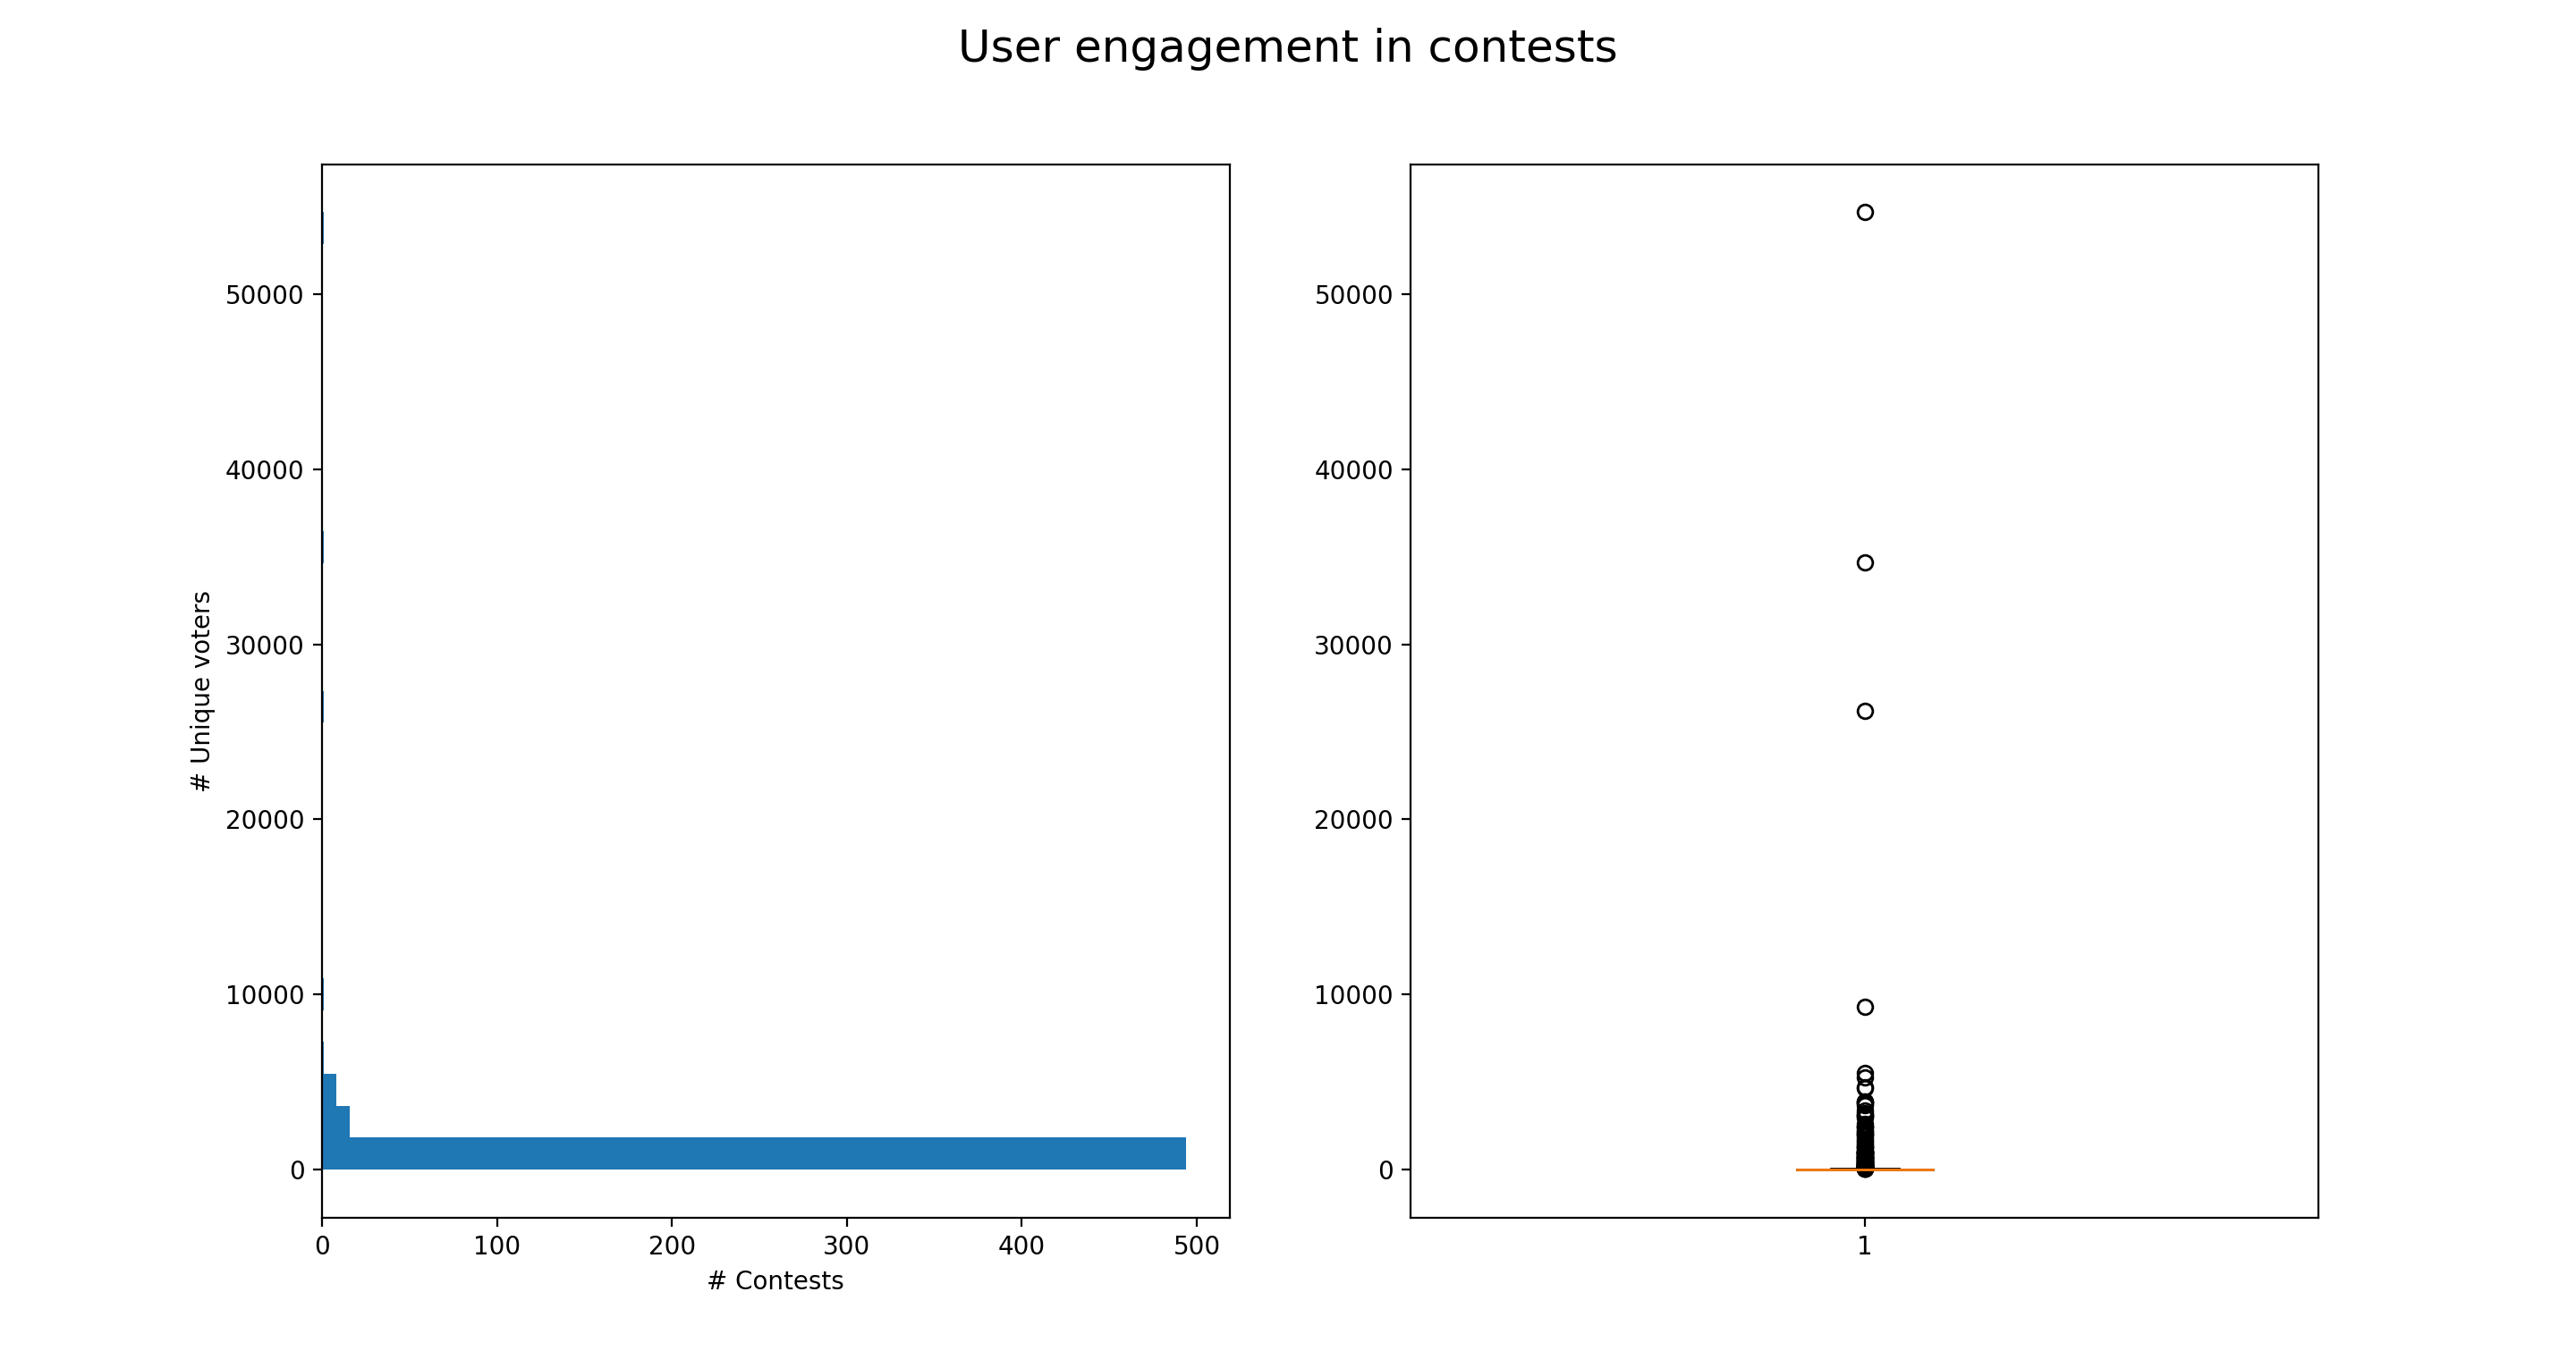
\includegraphics[width=0.8\textwidth]{Images/user_engagement_in_contests.png}
            \caption{The number of unique voters over contests.}
            \label{user_engagement_in_contests}
        \end{center}
    \end{figure}

    It can be easily seen that most of the contests engage very small amount of users, as the median of the unique voters value for all contests is 3. However, some of the contest have proven to be very successful, as the highest number of unique voters is close to $max_{unique_voters} \approx 55 000$. This observation is also supported with the mean value ($\mu = 464.65$) and the standard deviation ($\sigma = 3111.44$). 
    
    The reason behind this observation can be explained by the fact that the customers did not establish a big user base yet. On top of that, many of the contests serve only testing purposes and engage only a few users. These findings suggests that contests with small enough unique voters should be excluded in the remainder of the analysis, because such observations are not representative and may create bias in the data.
    
    It can be seen from the histogram on Figure \ref{user_engagement_in_categories}, that a fairly high number of contests ($\approx 14 \% $) are categorized under the "other" category. This is probably due to the fact that authors did not assign the categories for one reason or another. It can be also seen that the amount of "beauty" and "fashion" contest is considerably high compared to the other categories, which is in align with the case company's profile at the point of conducting this study. From this visualization it is also visible that the amount of "sports" contests is considerably low ($\approx 3.5 \% $). After filtering out contests with only to the "other" category, it was identified that many of the sports, humor, design, beauty and fashion-related contests were indeed not labeled correctly in terms of their categories. This issue was fixed manually in the preprocessing phase. 

    % number of contests in overall, by category
    % explain the findings that there were too many "other" type of contests which were fixed manually
    \begin{figure}[h] 
        \begin{center}
            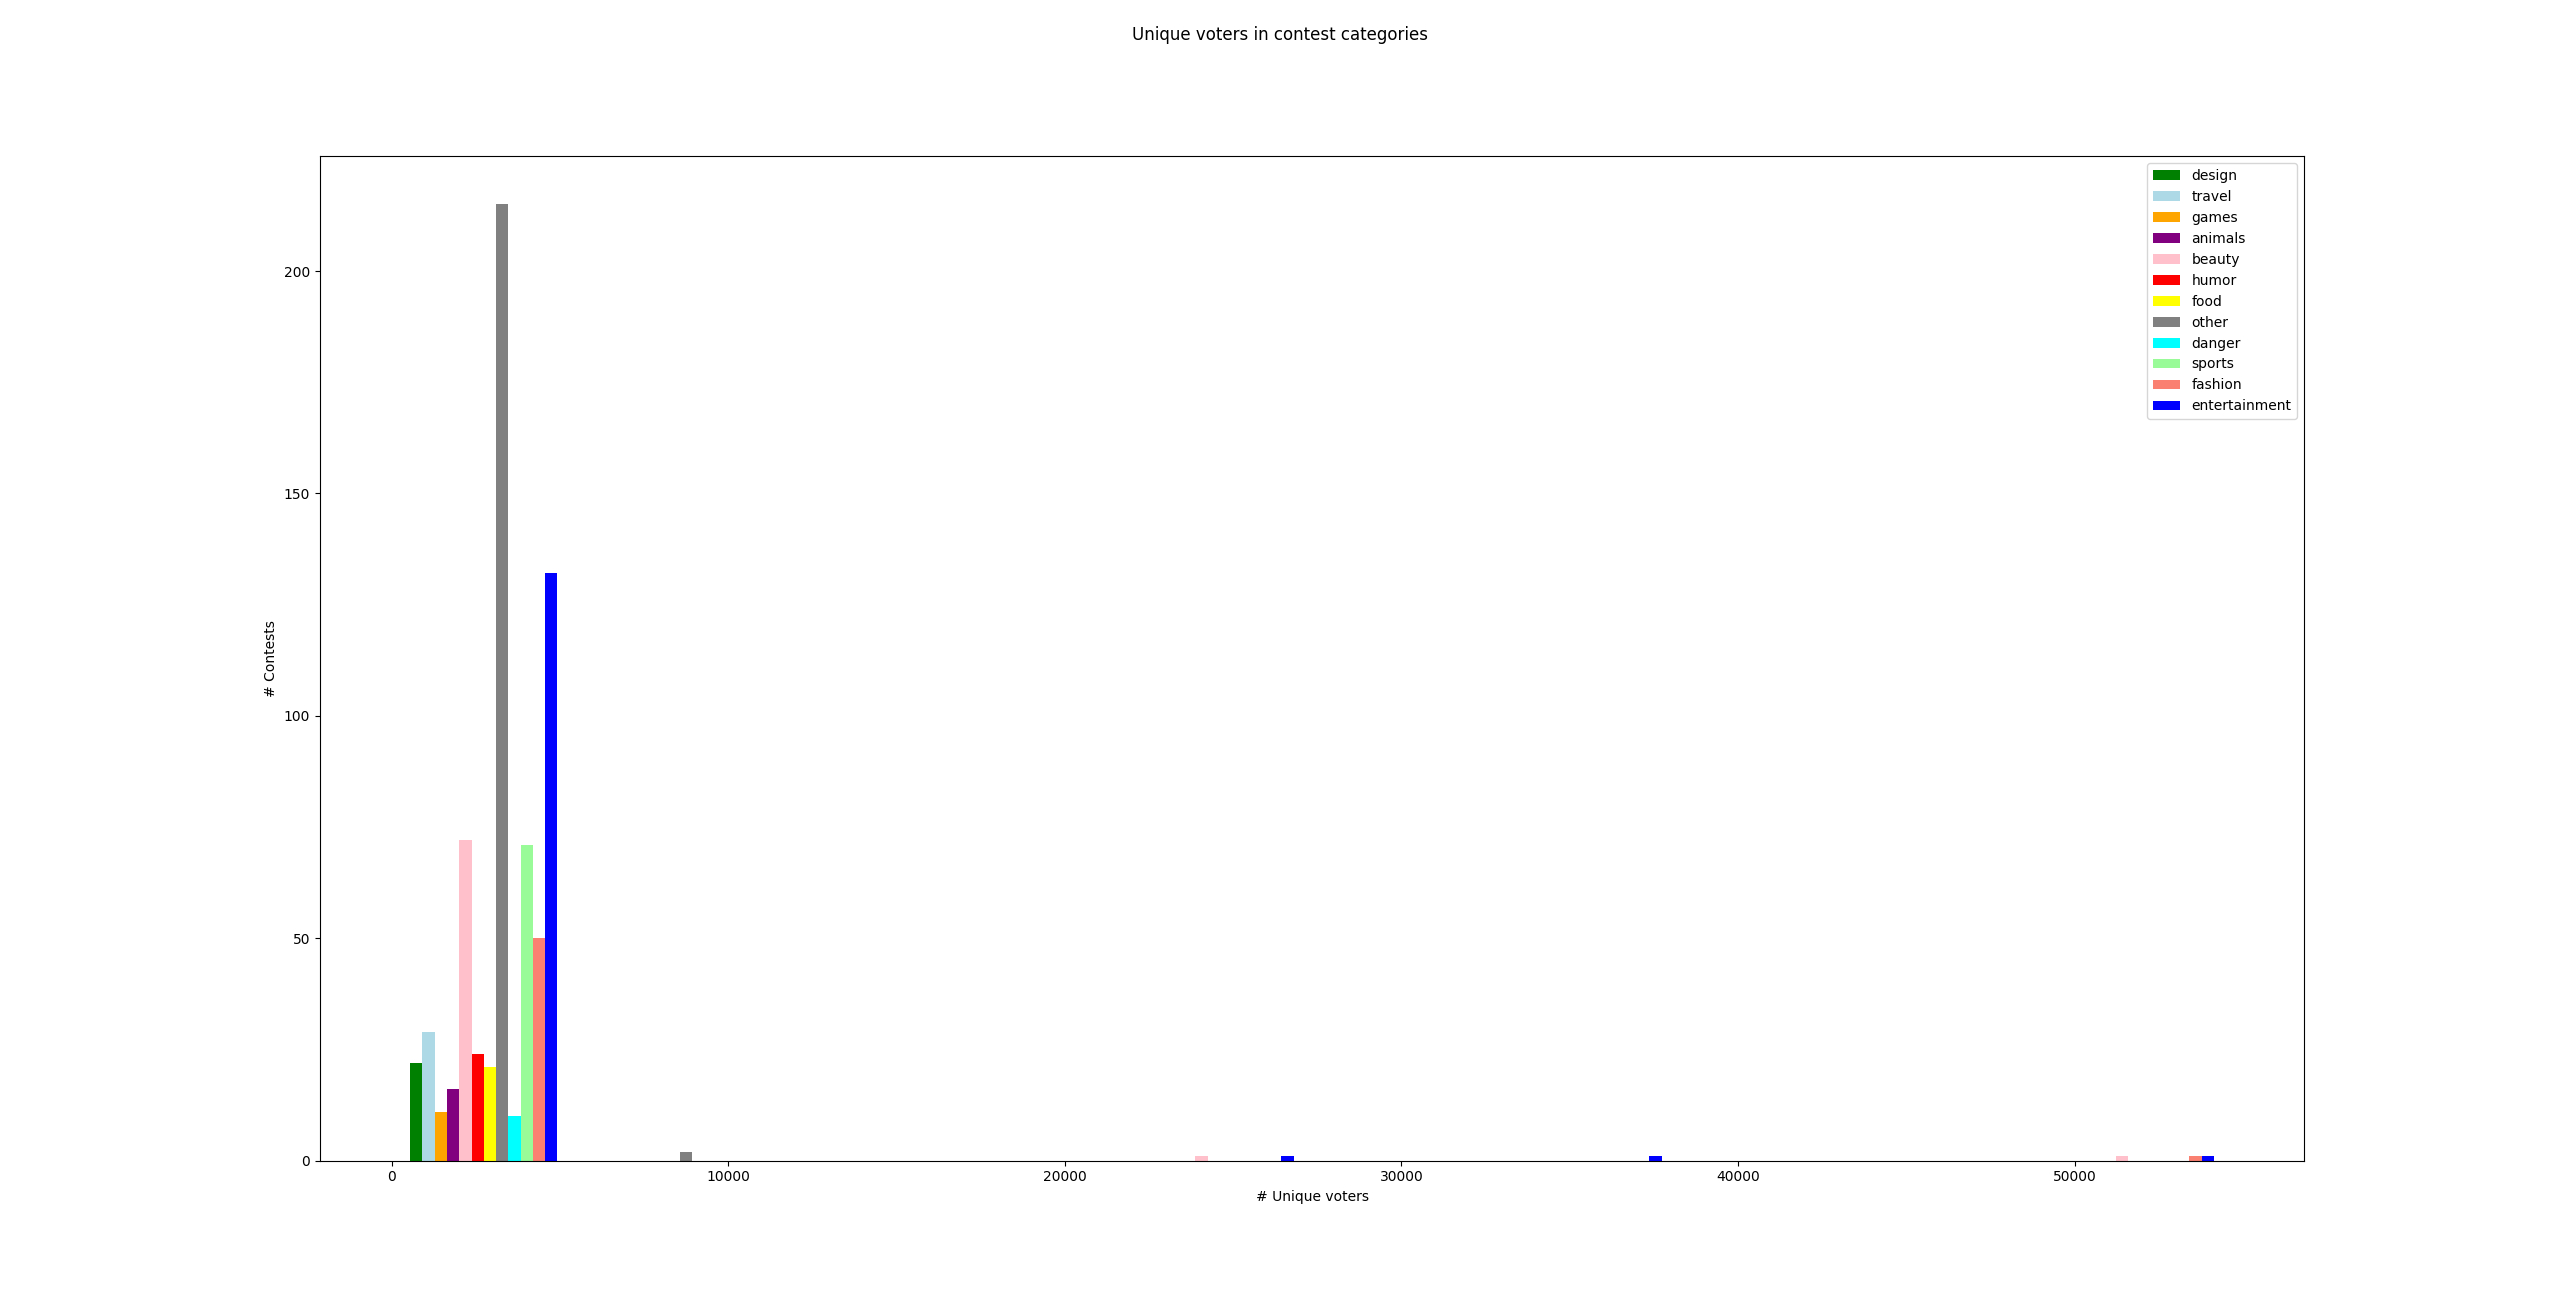
\includegraphics[width=0.8\textwidth]{Images/user_engagement_in_categories_bar.png}
            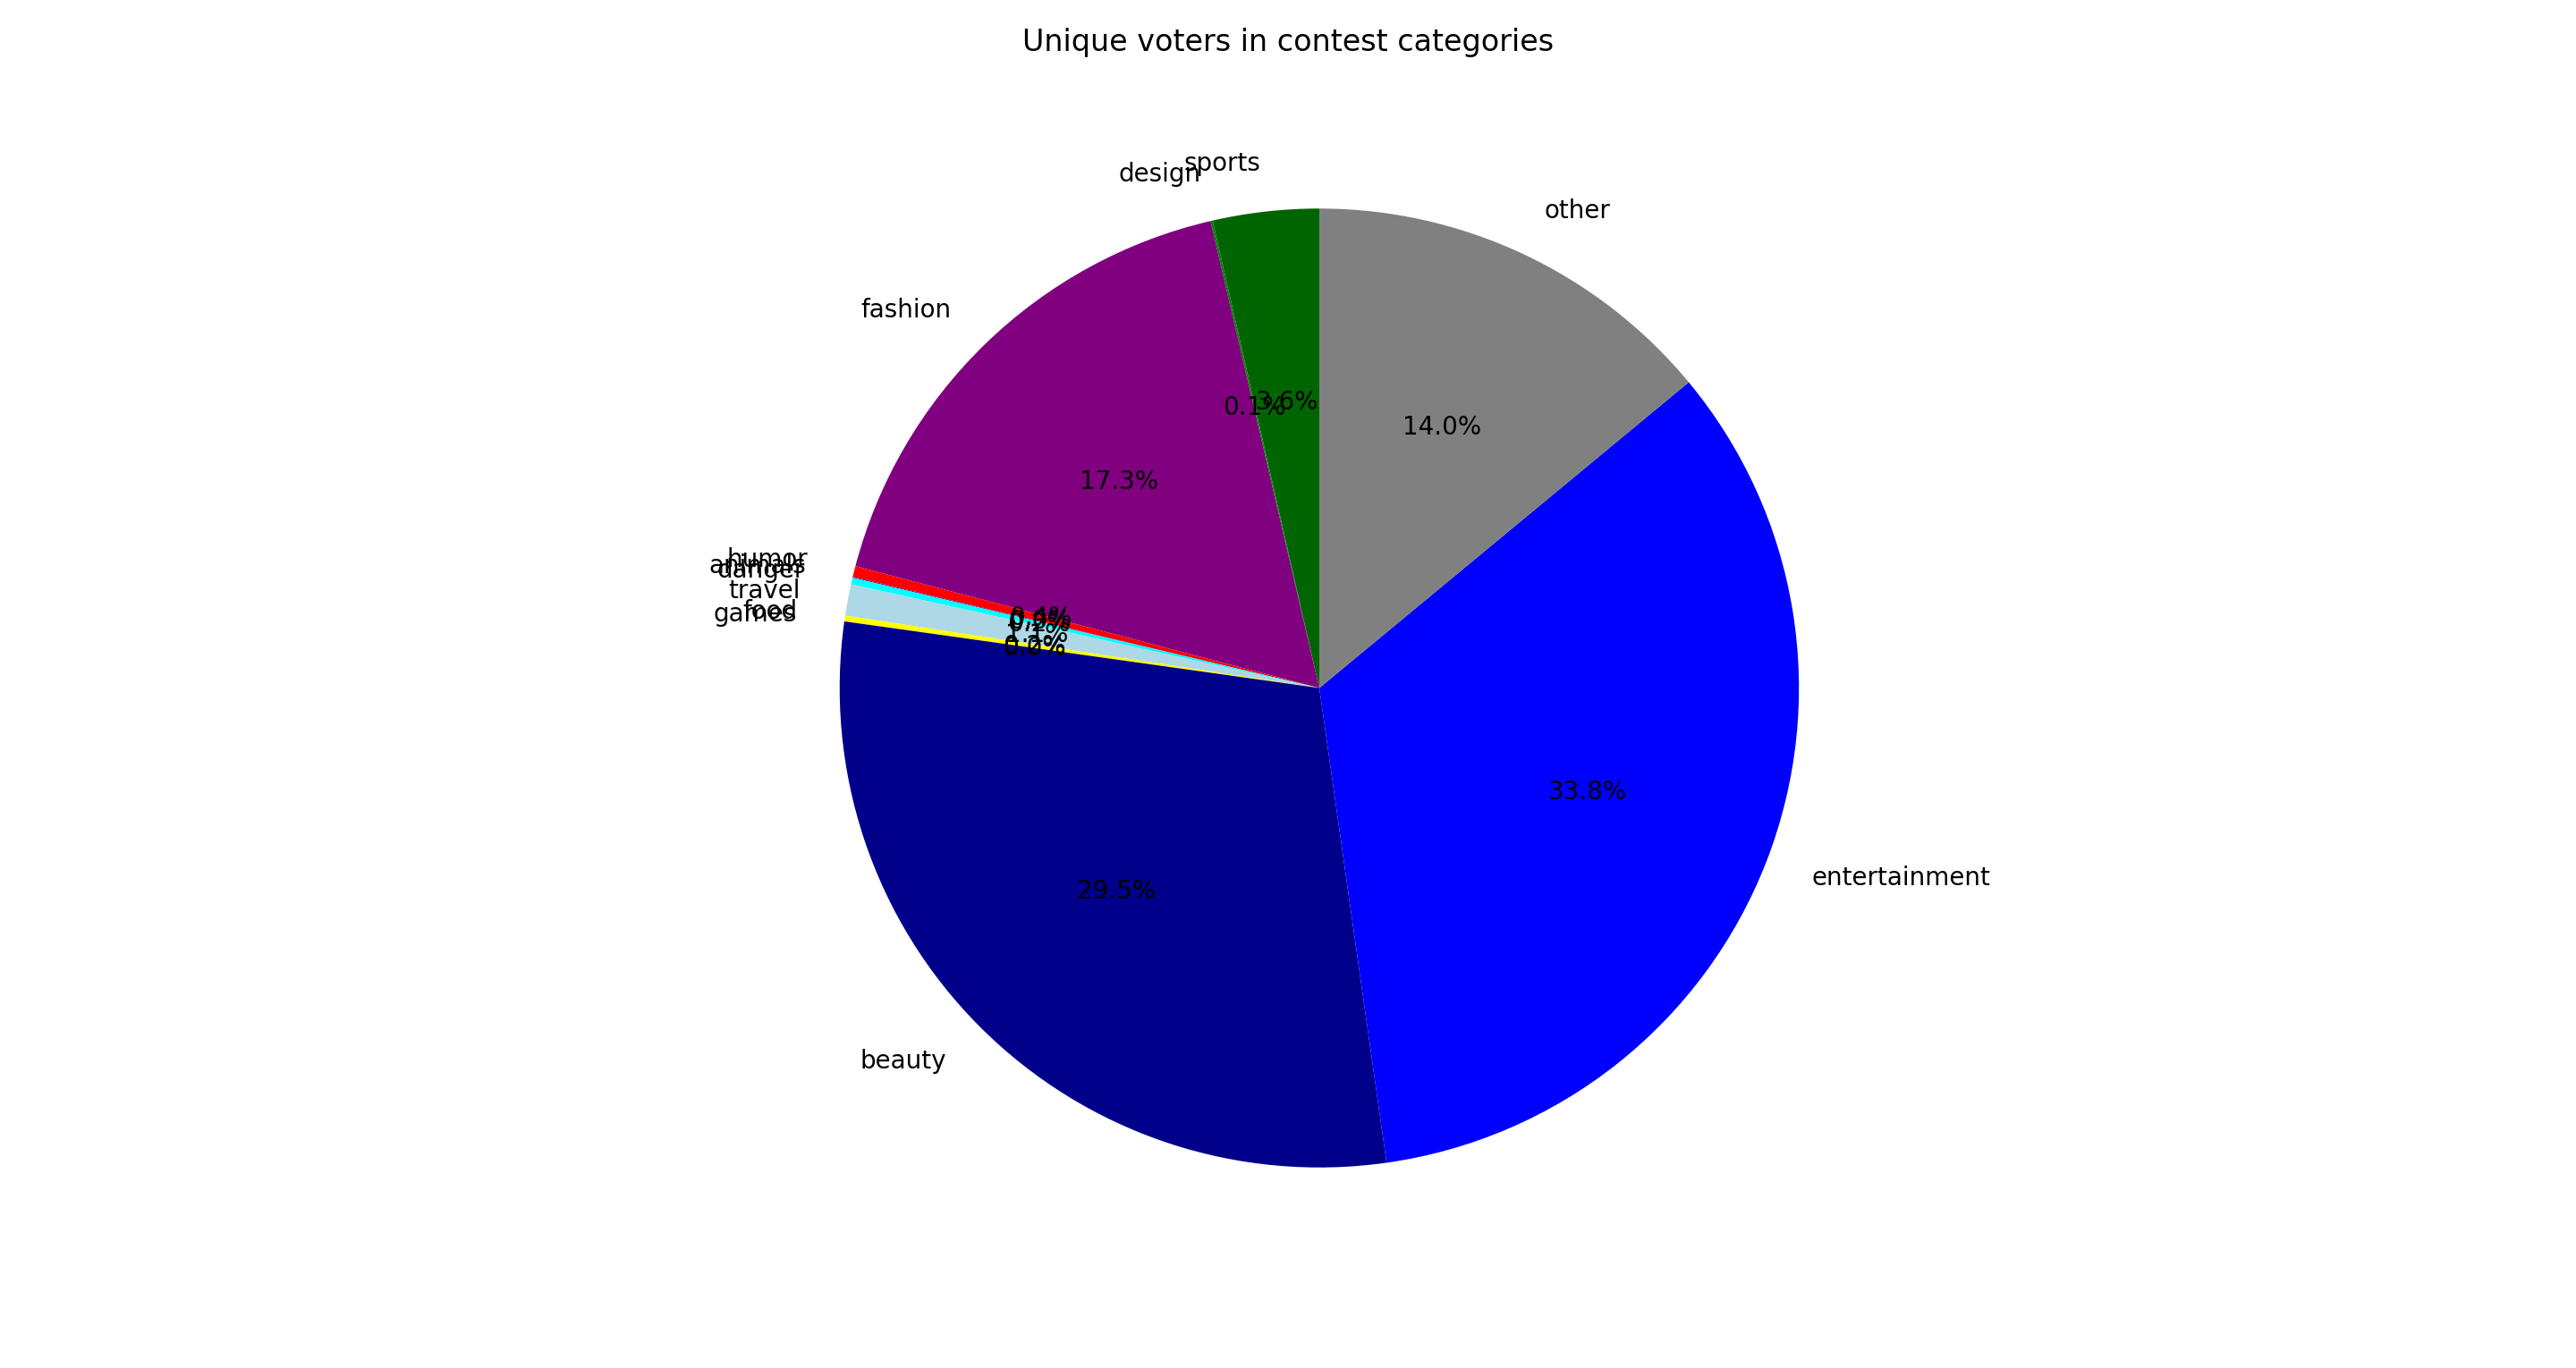
\includegraphics[width=0.8\textwidth]{Images/user_engagement_in_categories_pie.png}
            \caption{The number and percentage of unique voters over categories.}
            \label{user_engagement_in_categories}
        \end{center}
    \end{figure}

% explain the distribution of users by gender, age group and country
% Figure \ref{user_demographics_distribution} shows the distribution of 140 900 user profile in terms of gender, age group and country. This data is retrieved through each users profile, if they have given the related information or the privacy settings of the social media authentication allowed to retrieve the data. In case the information was not given or available from the social media profile, each filled was filled up with "other" values. It can be seen from the figure, that the distribution of males and females is considerably equal in the Choicely platform, but there is a large number of users, whose gender is unknown. Similarly, age group of users is often not known, however it can be seen that younger users are more active in Choicely, while elderly visitors are less engaged. 
% % TODO: explain nationalities as well in case anything interesting is gonna be done with them

% \begin{figure}[h] 
%     \begin{center}
%         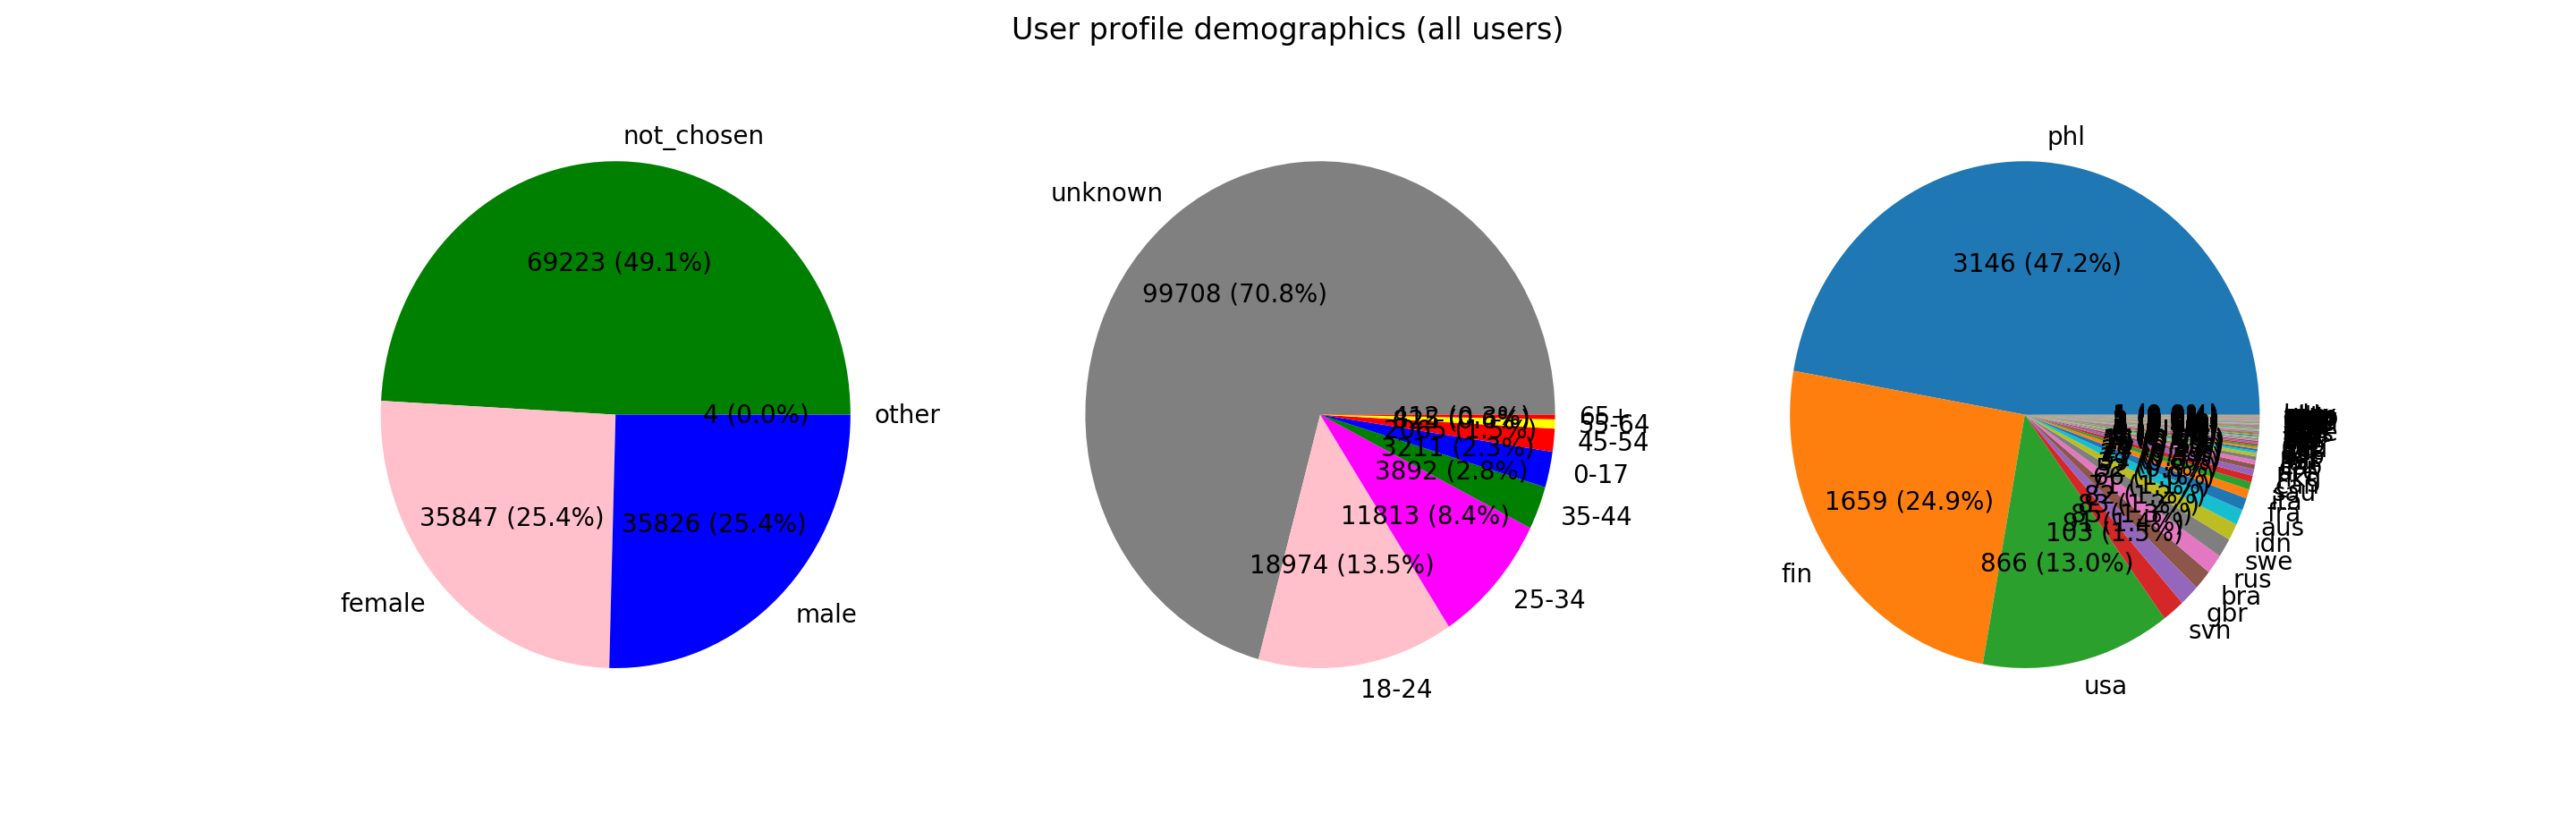
\includegraphics[width=0.8\textwidth]{Images/user_demographics_distribution.png}
%         \caption{The distribution of demographic attributes over all users.}
%         \label{user_demographics_distribution}
%     \end{center}
% \end{figure}

% compare to the distribution of users who have participated in more than 2 contest -> compare and elaborate   
It was studied how often users return to participate in more than one contests. After retrieving all user profiles and their votes over all contests, the users who participated in less than 2 contests were filtered out. Figure \ref{user_demographics_distribution-pruned} displays the demographic attributes of such users. It can be seen that only a very small portion ($3362 / 140900 = 2.4 \% $) of the users return to participate in more than two contests. Interestingly however, $46.2 \%$ of the returning users are females, which is a big difference compared to their ratio in the overall population ($25.4 \% $, Figure \ref{user_demographics_distribution}). It allows the conclusion that females tend to be more active in terms of returning to vote in multiple contests. 

\begin{figure}[h] 
    \begin{center}
        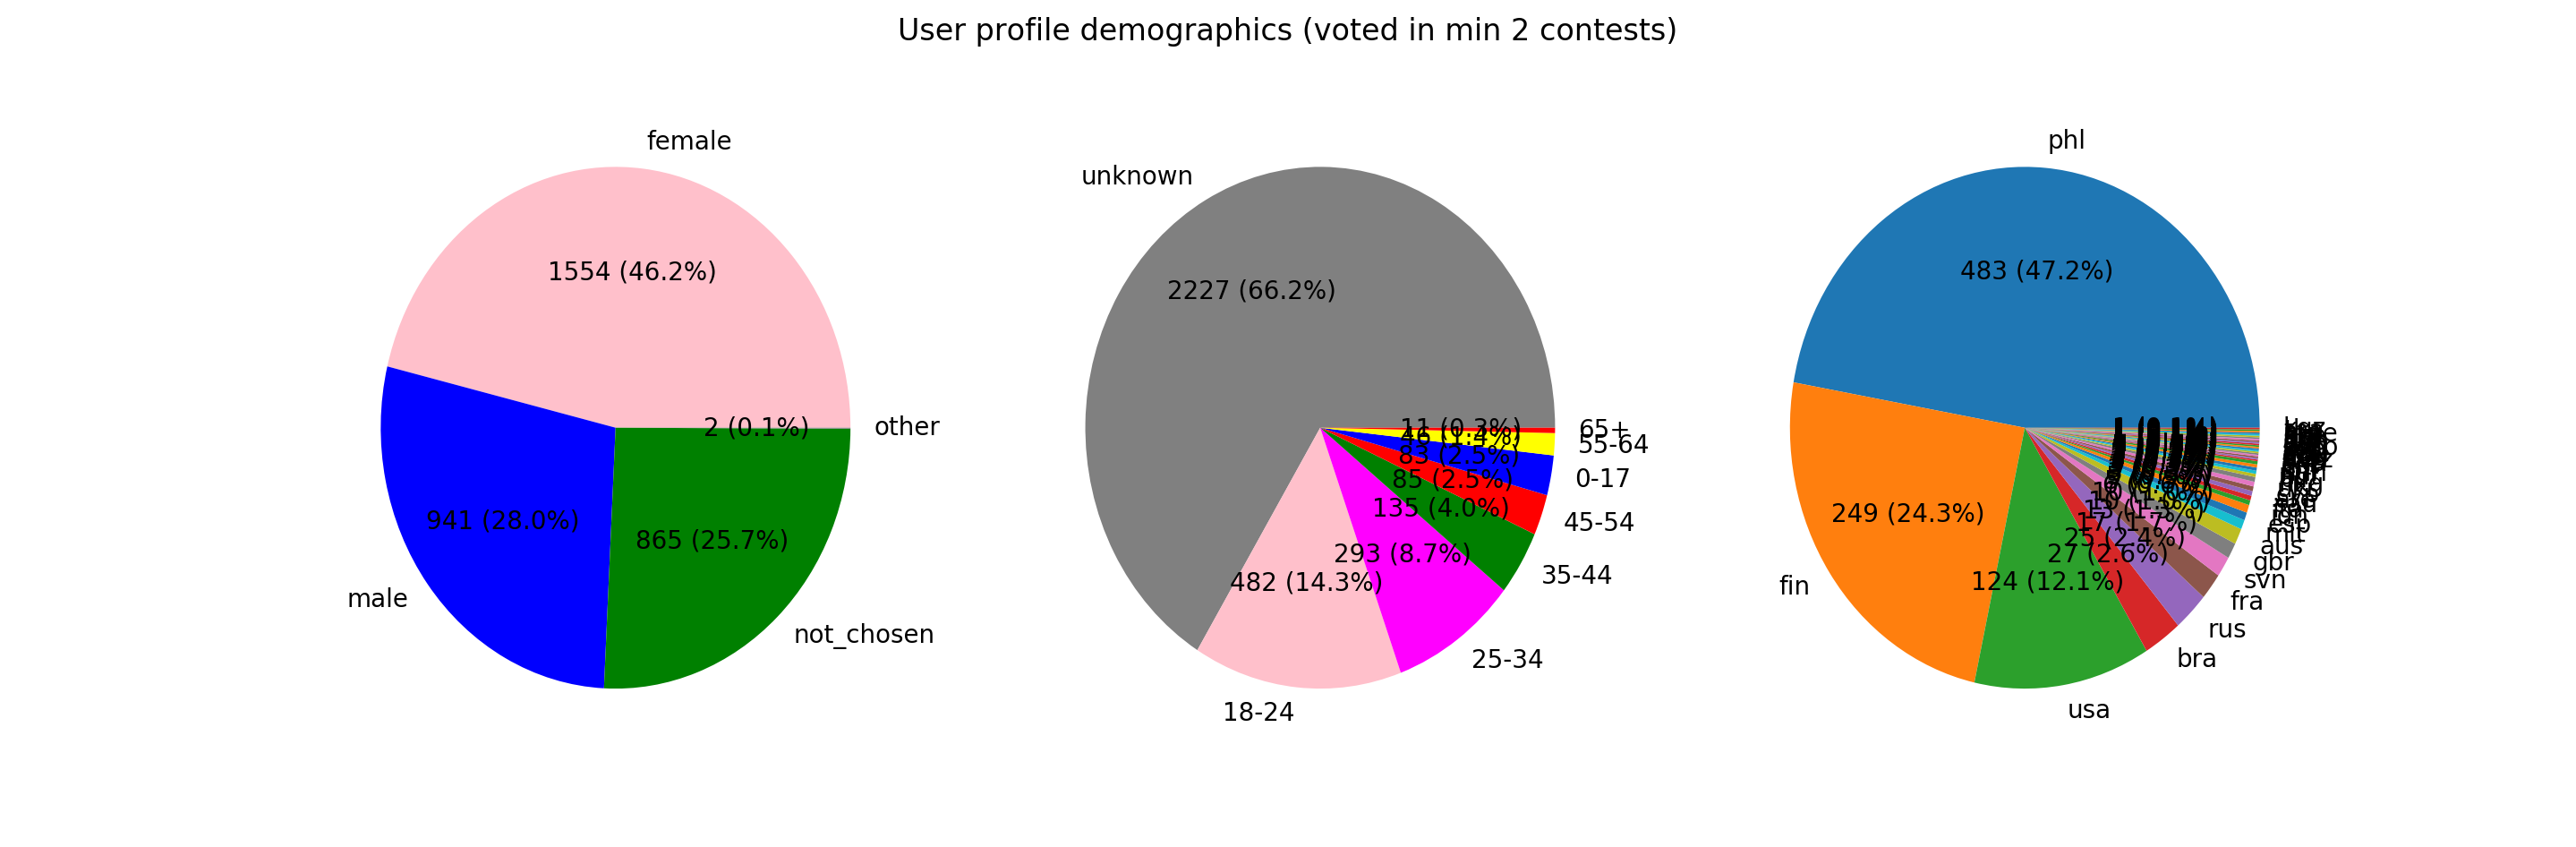
\includegraphics[width=0.8\textwidth]{Images/user_demographics_distribution-pruned}
        \caption{The distribution of demographic attributes over users who have participated in at least 2 contests.}
        \label{user_demographics_distribution-pruned}
    \end{center}
\end{figure}

% sum up and conclude
The EDA has highlighted multiple ways how the data should be pruned in order to ensure the relevance of the data. (...)
% TODO Conclusion

\subsection{Preprocessing and pruning}
It was identified, that some of the data cannot be used for the purposes of this study and the results will be more representative, if some of the data is pruned. 

% contests
\begin{figure}[h] 
    \begin{center}
        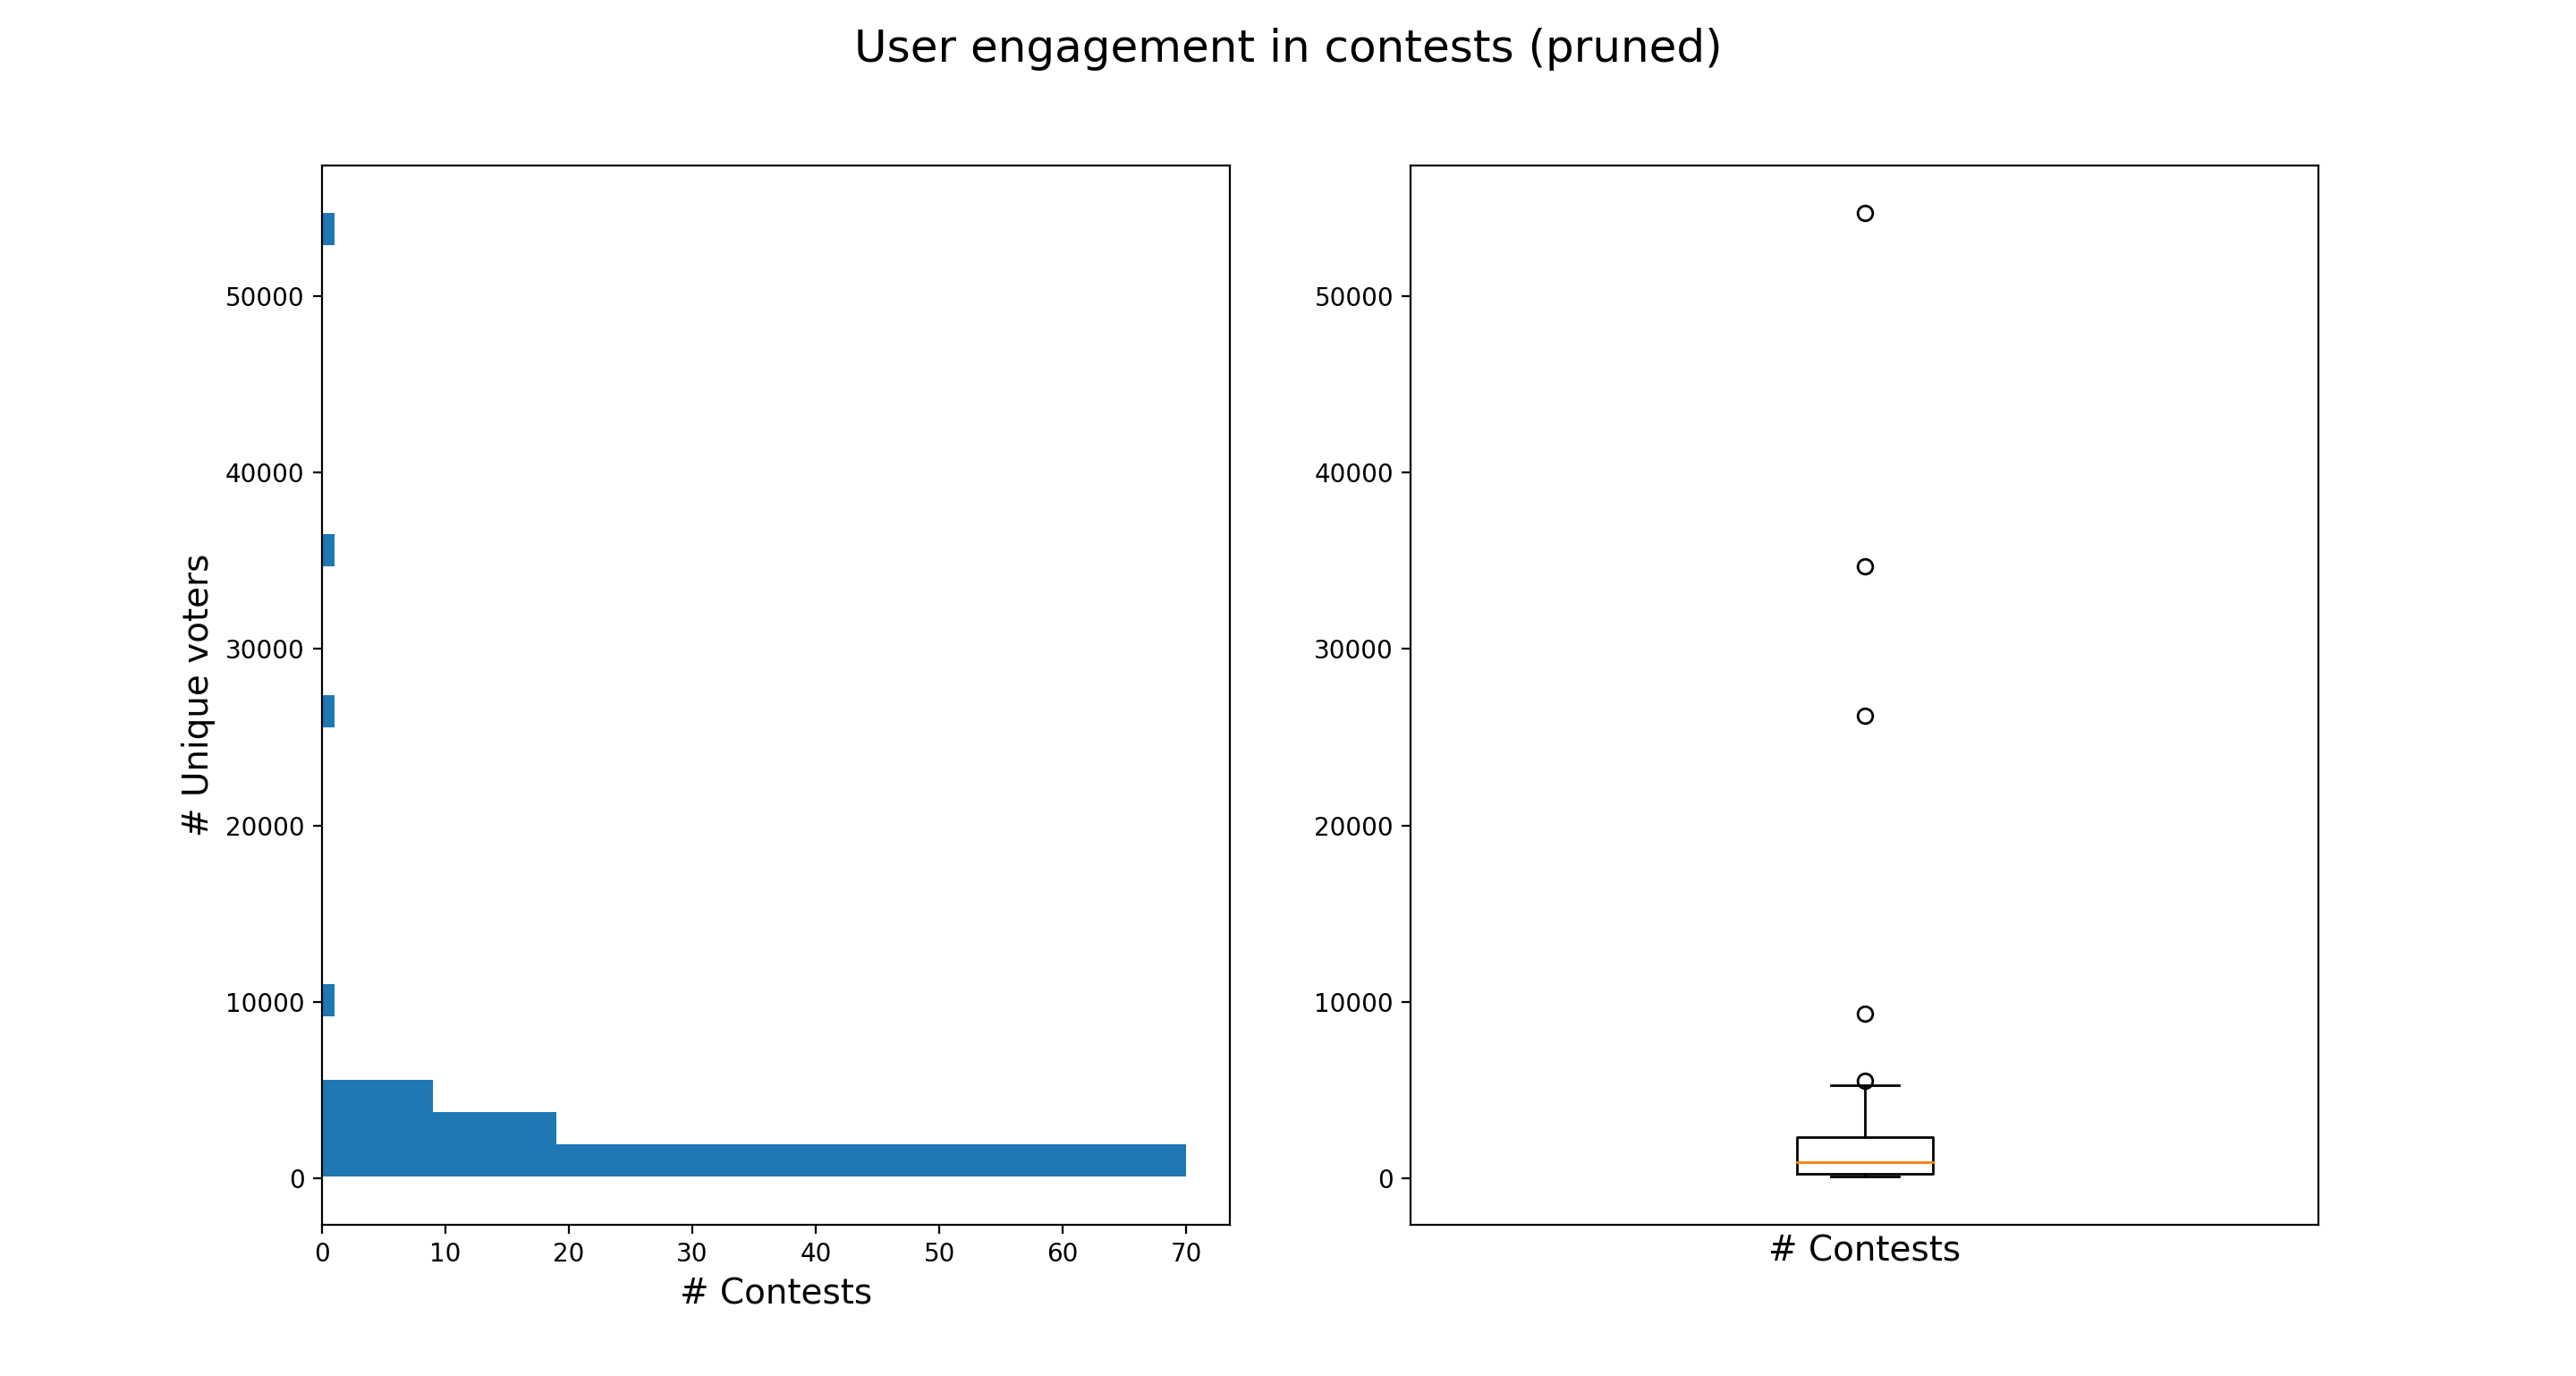
\includegraphics[width=0.8\textwidth]{Images/user_engagement_in_contests-pruned.png}
        \caption{}
        \label{}
    \end{center}
\end{figure}

\begin{figure}[h] 
    \begin{center}
        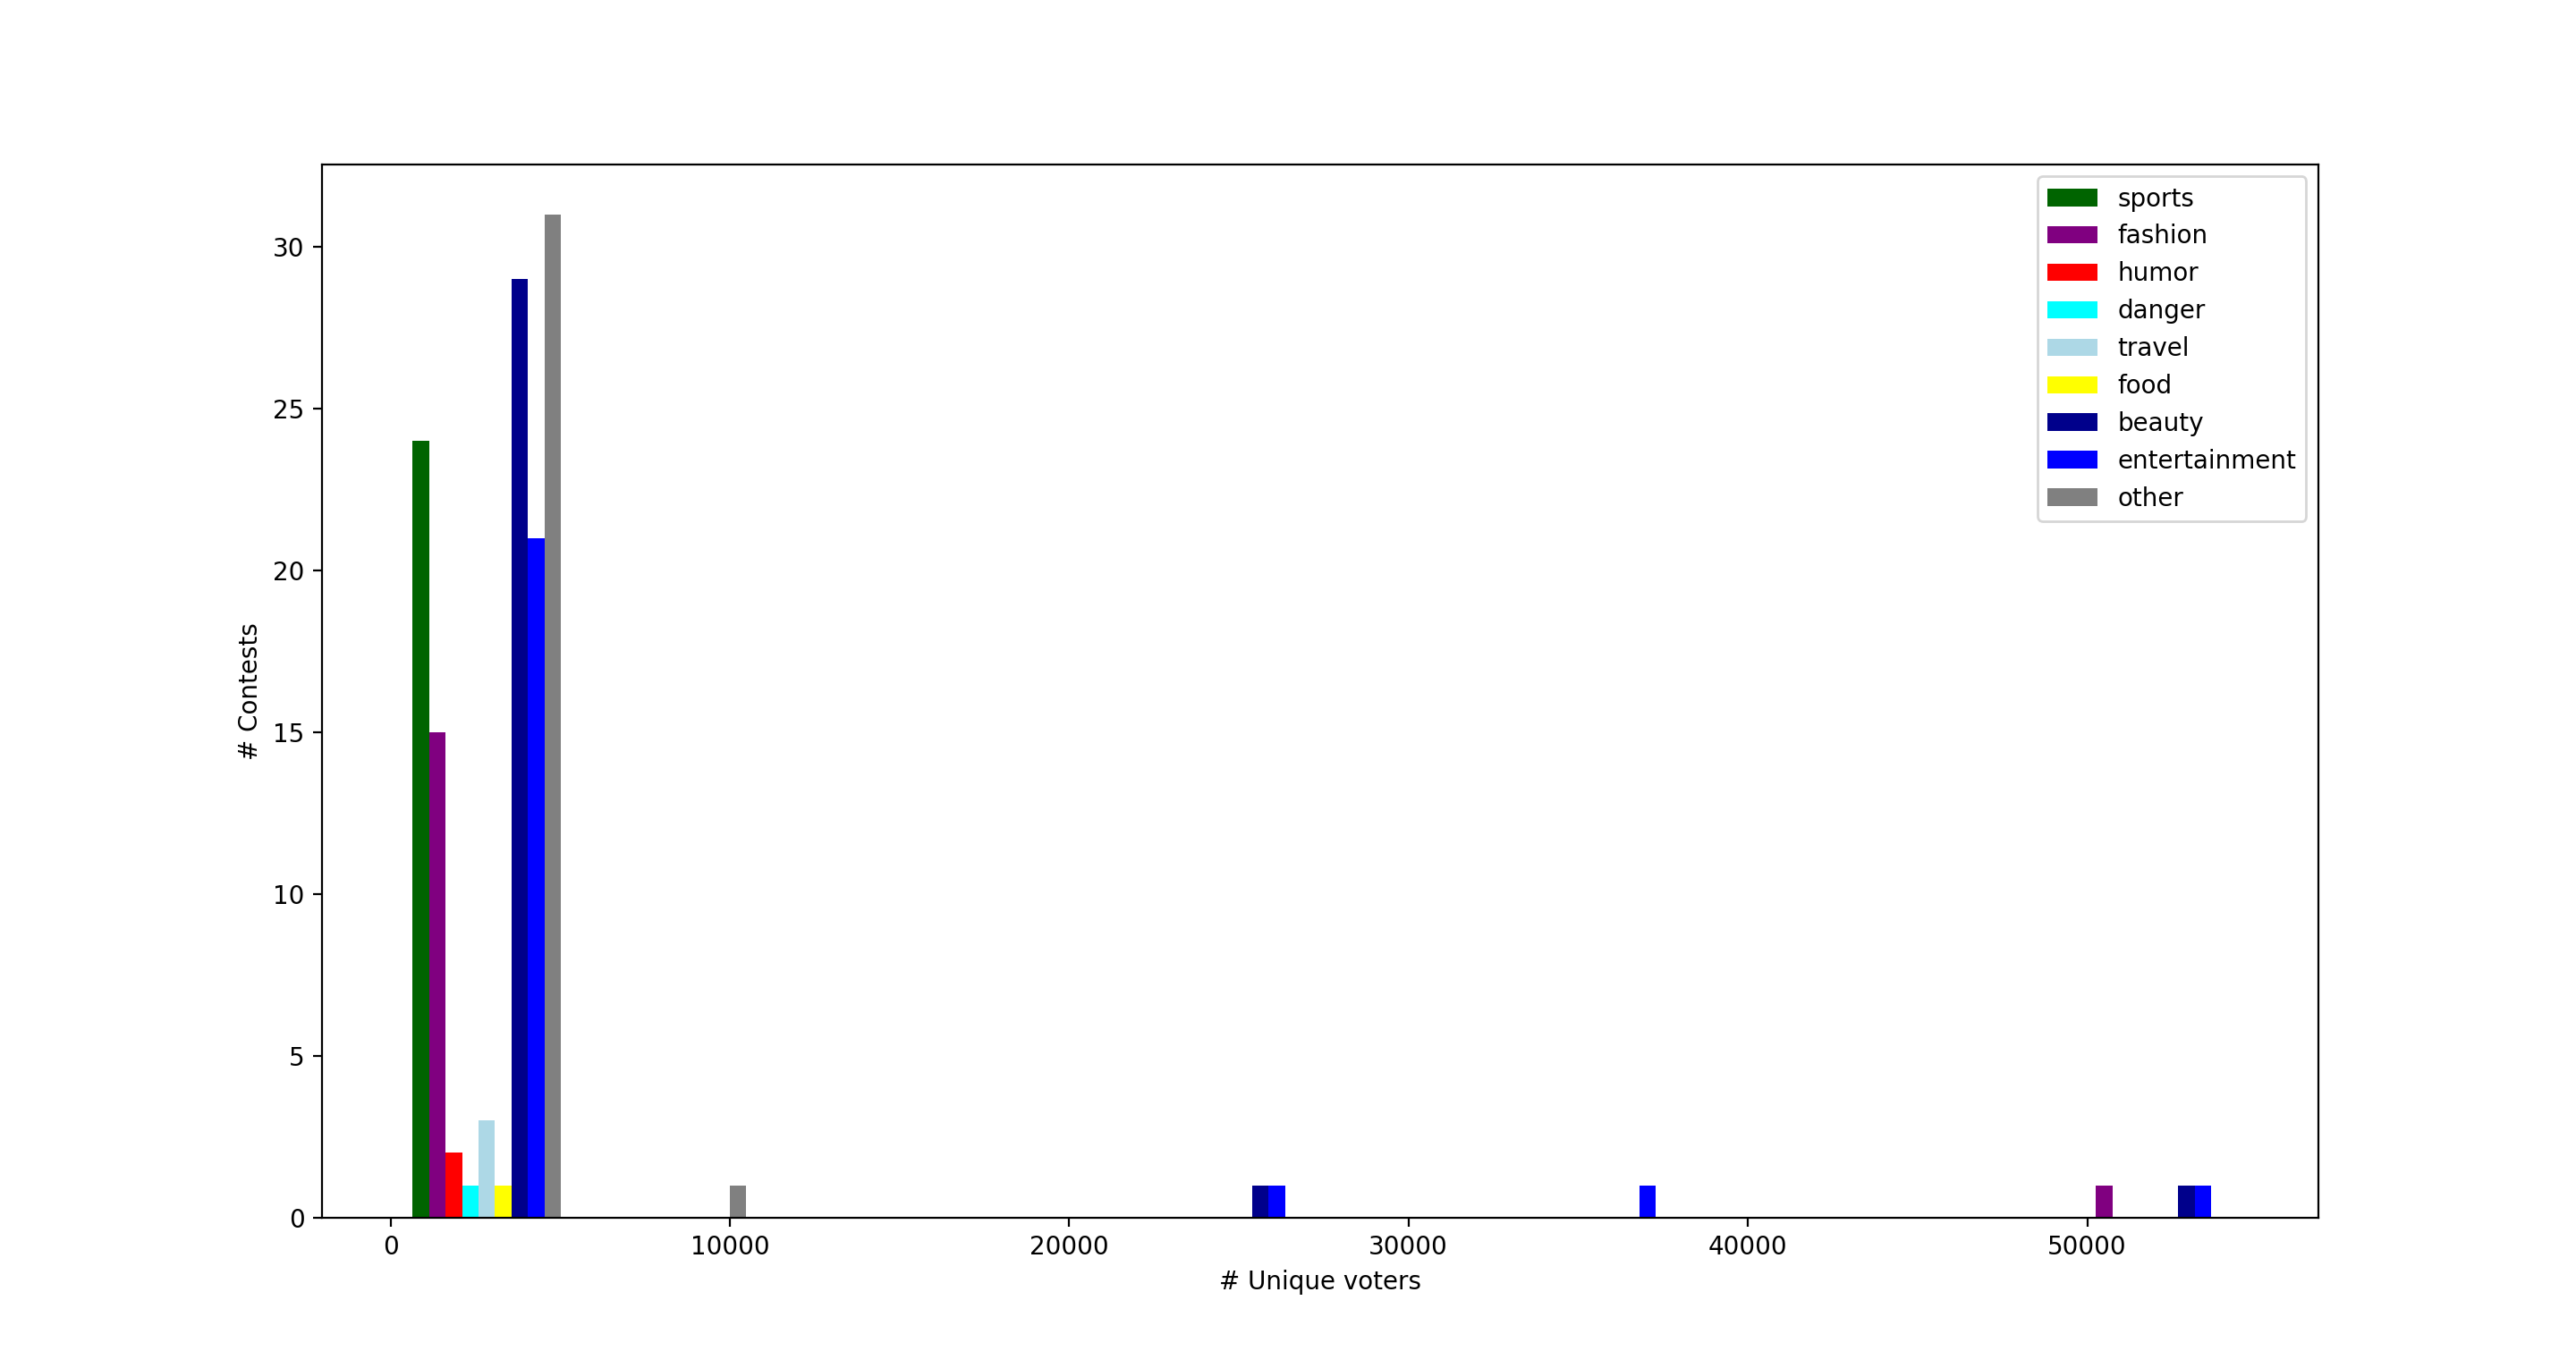
\includegraphics[width=0.8\textwidth]{Images/user_engagement_in_categories_bar-pruned.png}
        \caption{}
        \label{}
    \end{center}
\end{figure}

\begin{figure}[h] 
    \begin{center}
        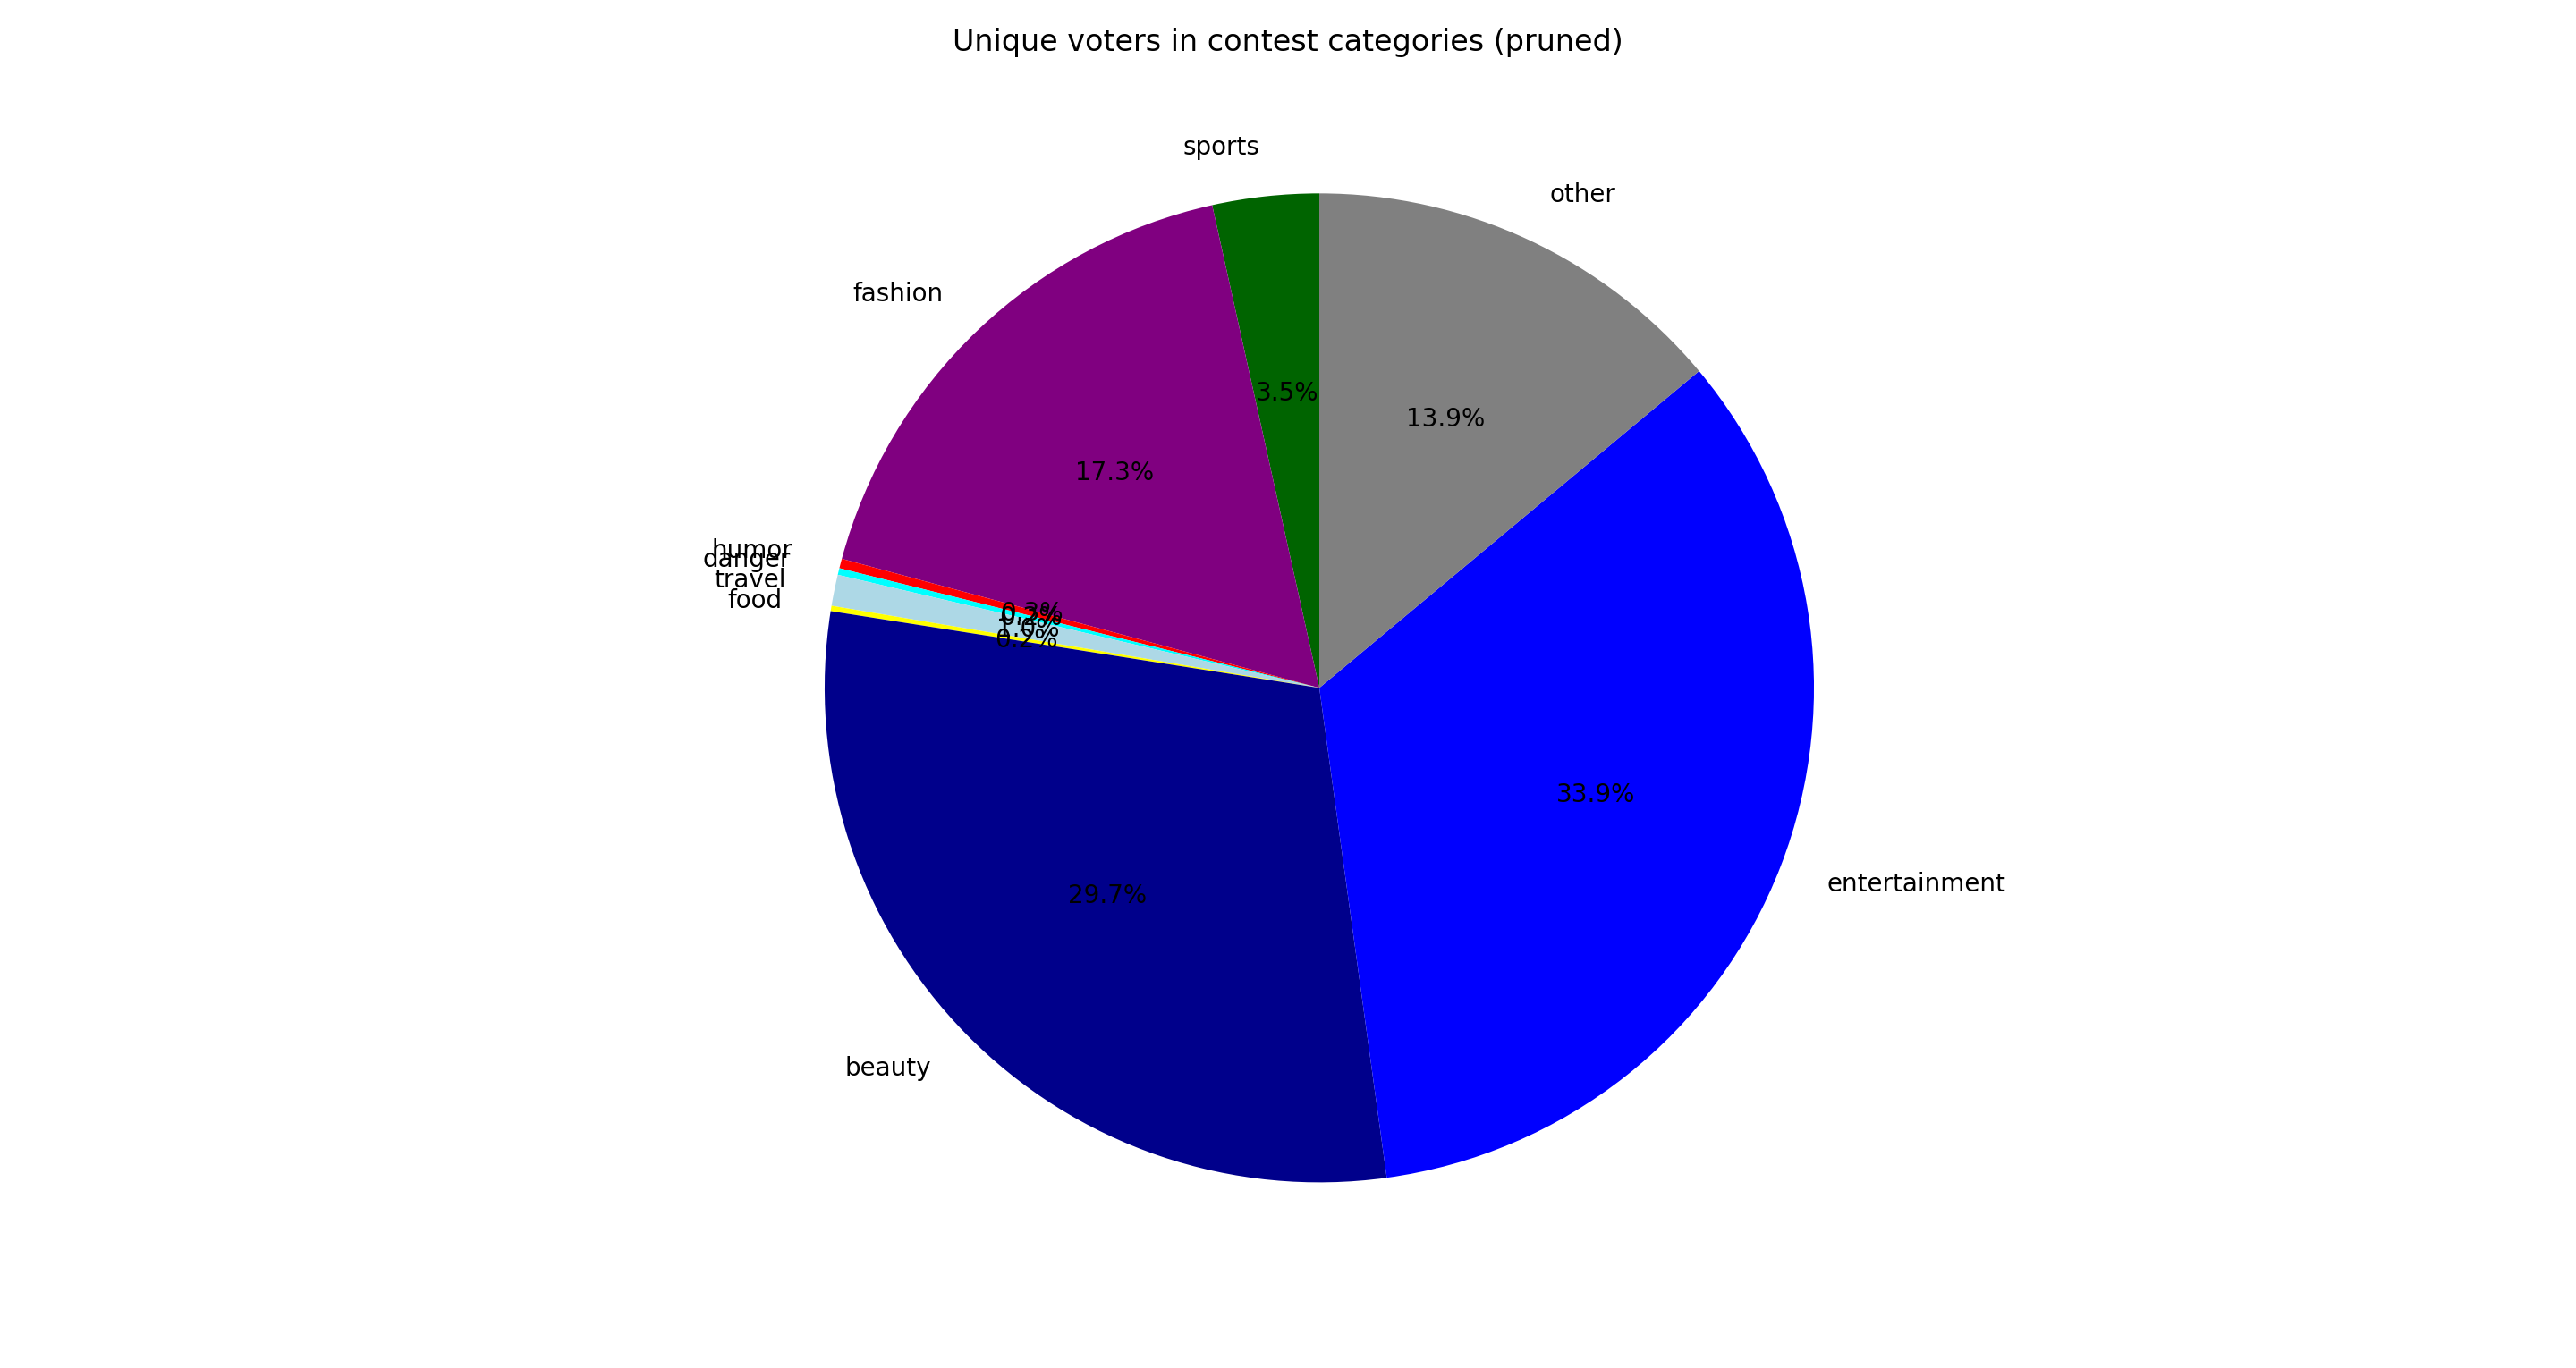
\includegraphics[width=0.8\textwidth]{Images/user_engagement_in_categories_pie-pruned.png}
        \caption{}
        \label{}
    \end{center}
\end{figure}
% users

% Entities that match any of the rules displayed in Table \ref{preprocessing_rules} are dropped from the analysis. For instance, contests with less than 100 unique voters (users) and images without labels are considered irrelevant, and may bias the results of the study. After applying the preprocessing rules, the dataset is left with 92 contests, 1625 contest participants, 282545 votes and XXX unique voters over 10 contest categories. % TODO update occasionally

\subsection{Association analysis}
